%\documentclass{article}
%\usepackage{graphicx,subfigure}
%\begin{document}

\begin{figure}[!h]
  \centering
  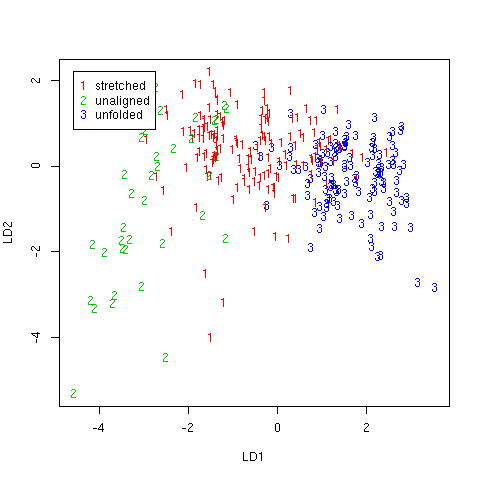
\includegraphics[width=1.1\textwidth]{figldaall.png}
  \caption{Plot of discriminant functions LD1 and LD2 which are the two dimnsions used to discriminate CrimpTypeFM classes. Each point is the LD1 and LD2 function values for one sheep from the learning data set of 340 sheep. The three CrimpType FM classes are shown as colours and numerals}
  \label{fig:ldaall}
\end{figure}

%\end{document}

